\section{Data Processing}
As mentioned earlier, Python was chosen for data processing. Python has an established data analysis community, and as such provides a rich assortment of open-source libraries that can be used. With a such a community, documentation was abundant and meant that the implementation of the designs discussed in Chapter \ref{Chapter:Design} were accelerated greatly. Not only this, but existing solutions for problems encountered during development were available, which again sped up the implementation process. 


\subsection{Abuse Detection}
This is a single-class classification problems. The challenge is to detect when a comment from a conversation would be considered insulting to another participant in the conversation. The idea is to create a generalisable single-class classifier which could operate in a near real-time mode. Classification is a form of supervised learning, it takes a set of data ${X, Y}$ where $X$ is a set of attributes and $Y$ is the target class. The goal is to model $Y$ as a function of $X$, $y = f(x)$, where $x \in X$ is a specific sample and $y \in Y$ is the corresponding class for that sample.

Abuse detection is primarily implemented in python, consisting of multiple scripts. The script requires python version 2.7 or above to executes due to certain dependencies and functions used. The script makes use of multiple Python libraries including Sci-kit learn \cite{scikit:home}, NLTK \cite{nltk}, Numpy \cite{Numpy} and Pandas \cite{Pandas}, and others such as mysql, which provide machine learning models and objects for loading and processing the data. The code for this functionality has been modularised and is thus split across various files and classes. This allows modules to be included, instantiated, upgraded and reused whenever necessary.

\subsubsection{Data Description}
As mentioned previously, classification is a form of supervised learning. This means that a dataset is required to train the classifier which can then be used to make predictions on unseen instances, based on the training data. A suitable dataset was found online, provided by Impermium and hosted on the popular machine learning competitions site Kaggle \cite{Kaggle:Dataset}. The dataset was split into two files, train.csv and test.csv, and consisted of three attributes: Insult, Date, Comment. The training set contains 3,948 samples and would be used to train the models whereas the test set contains 2,648 samples and would be used to verify the accuracy of the model.


\subsubsection{Data Preprocessing}
As the data has been downloaded from a third-party, we must ensure that it is in the correct format. The data preprocessing stage will ensure that all the training and test data is consistent with the data we expect on the social network. This step is only carried during the training phase.

 The dataset was loaded into memory as a table (DataFrame) using the Pandas library. The library provided a function to read csv files with headers as demonstrated in figure \ref{fig:AbuseDetection_LoadData}. A generic function was created for loading in the dataset as this functionality is required multiple times, for loading the test and training datasets separately.

\begin{figure}[H]
	\centering
	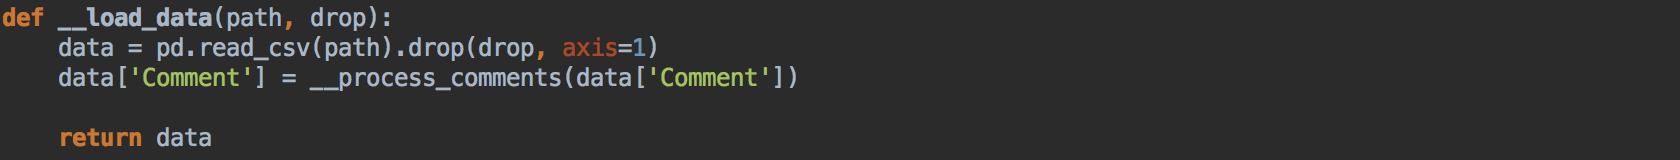
\includegraphics[width=\textwidth]{Images/Implementation/DataProcessing/AbuseDetection/LoadData}
	\caption{Function that cleans a post}
	\label{fig:AbuseDetection_LoadData}
\end{figure}

The raw dataset contains multiple errors which will effect the accuracy of the resulting model. As a result, before the data can be used, it needs to be processed and cleaned. For example, there are comments which contain several ascii characters that have been encoded. Similarly, there are several comments which contain underscores and new line characters that must be stripped so the ngrams can be generated correctly.

\begin{figure}[H]
	\centering
	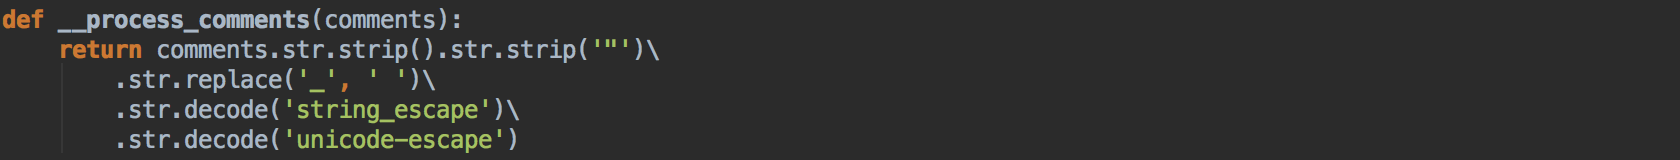
\includegraphics[width=\textwidth]{Images/Implementation/DataProcessing/AbuseDetection/ProcessComments}
	\caption{Function that cleans a post}
	\label{fig:AbuseDetection-ProcessComments}
\end{figure}

The function in figure \ref{fig:AbuseDetection-ProcessComments} processes the entire DataFrame in one go, firstly stripping any white space on the edges, then replacing all the underscores with spaces. The resulting string is then first decoded using string\_escape, which produce a string that is suitable as string literal in Python source code and then decoded using unicode\_escape, which produce a string that is suitable as Unicode literal in Python source code \cite{Python:Codes}.

\begin{figure}[H]
	\centering
	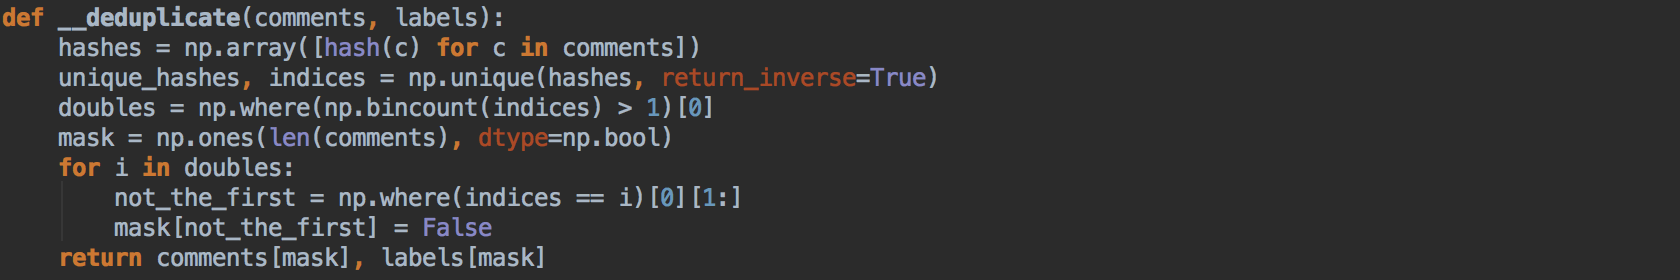
\includegraphics[width=\textwidth]{Images/Implementation/DataProcessing/AbuseDetection/Deduplicate}
	\caption{Function that cleans a post}
	\label{fig:AbuseDetection-Deduplicate}
\end{figure}

The next step involved cleansing the data by removing any duplicate comments in the training set. The function in figure \ref{fig:AbuseDetection-Deduplicate} takes a set of comments and their labels to filter out duplicated comments, returning only unique comments with their associated labels. The first part of this process computes the hash of every comment. This will result in the same hash for two comments that are identical, due to the nature of the hashing process. Next, we take the indices of all the unique hashes, which returns bins containing the indices corresponding to every hash value. As a result, if a hash appears twice then it will contains two indices in its bin. The indices of the hashes are then used to find the duplicates where the bin has more than indices in it. Given all the duplicates, we can generate a mask, lines 5-8, which only returns one instance of every duplicate comment. Finally, the mask is used to access all the unique comments and their associated labels.

\subsubsection{Feature Engineering}
In order to achieve a reasonable accuracy, the features of the dataset must be transformed into something meaningful.

\subsubsection{Modelling}

\subsubsection{}

SVC Accuracy: 0.767661708092


\subsection{Content Filtering}
The implementation of content filtering constitutes of Python scripts which handle all of the data preprocessing, training of the model and predicting of the post categories. The same Python libraries used for abuse detection are used here. The code is divided between three files, each of which handle a stage of the machine learning process: \emph{preprocess.py}, \emph{train.py} and \emph{predict.py}.

\subsubsection{Data Description}
Although in the future, Fidelis posts will be used to train the model, until there is sufficient data stored a training set from Twitter is used, as discussed in section \ref{sec:training-data}. This training set contains two attributes: tweet text and category. The categories correspond to the default main categories which are used on the discover page, which are: Arts, Business, Education, Games, Health, Home, News, Recreation, Science, Shopping, Society, Sport and Technology. There are 59010 tweets in the dataset. The graph in figure \ref{fig:category-spread} shows the distribution of tweets in each category, with Arts being the most prevalent with 6680 tweets and Shopping the least with 693 tweets.

\begin{figure}[H]
\centering
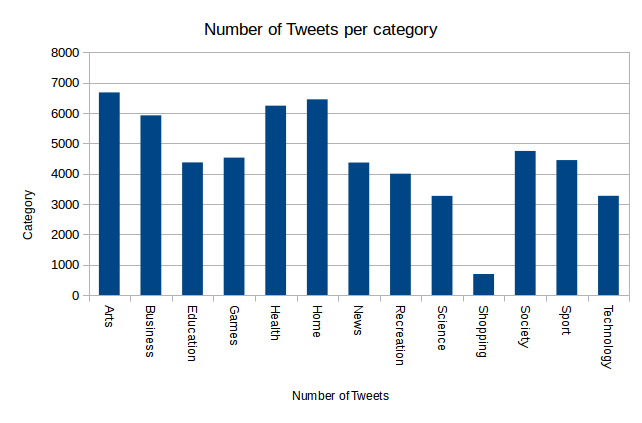
\includegraphics[width=\textwidth]{Images/Implementation/category-spread}
\caption{Spread of Tweets over categories in training set}
\label{fig:category-spread}
\end{figure}

\subsubsection{Data Preprocessing}
\textit{preprocess.py} cleans posts so that they can be used in either the training or predicting processes. The implementation of cleaning is shown in figure \ref{fig:content-clean}. The function carries out a list of commands sequentially, each of which remove aspects of the post which are unwanted. The package \textit{p}, from which the \textit{clean()} function is used, is the tweet-preprocessor package \cite{TweetPreprocessor}. This function removes any Twitter entities, except for the hashtags, from the post, including mentions, URLs and emoticons. Since Fidelis is using the same tagging system as Twitter, the same cleaning function can be applied to Fidelis posts. The $WordLemmatizer$ object is from the NLTK library, which processes lemmatized versions each of the words in the post to reduce the noise created as a result of different forms of the same word. 

\begin{figure}[H]
\centering
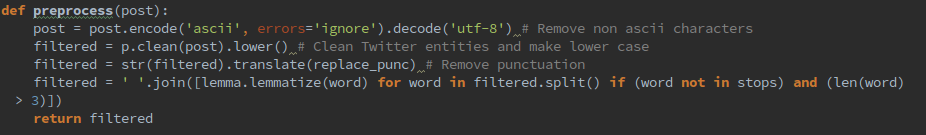
\includegraphics[width=\textwidth]{Images/Implementation/content-clean}
\caption{Function that cleans a post}
\label{fig:content-clean}
\end{figure}

The only part of algorithm \ref{alg:content-filter-cleaning} not performed by this function is the check on the length of the preprocessed string. This is instead performed by both the training and prediction functions. Figure \ref{fig:content-preprocess} shows the preprocessing which occurs in the training file.

\begin{figure}[H]
\centering
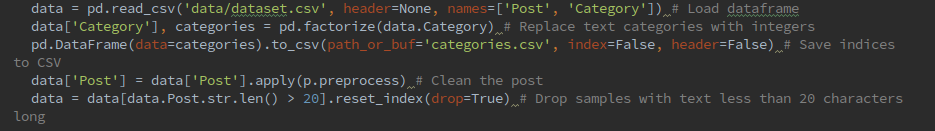
\includegraphics[width=\textwidth]{Images/Implementation/content-preprocess}
\caption{Preprocessing of content before training}
\label{fig:content-preprocess}
\end{figure}

The extraction of features from the post is conducted in the training and prediction files, because they are performed on the dataset as a whole rather than on each individual post. The count vectorization and TF-IDF transformations are parsed into the pipeline shown in figure \ref{fig:imp-content-train}, using the scikit-learn objects $CountVectorizer$ and $TfidfTransformer$. The $CountVectorizer$ also creates the uni- and bi-grams which are present in the dataset.

\subsubsection{Model Building}
Figure \ref{fig:imp-content-train} shows how the Stochastic Gradient Descent model is trained, including the pipeline which extracts features from the dataset. Whereas the pipeline stage creates the model, the \textit{fit()} function is what initiates the training of the model on the training data. As in section \ref{sec:exporting}, the trained models can then be exported so that they are usable for predicting incoming tags and posts.

\begin{figure}[H]
\centering
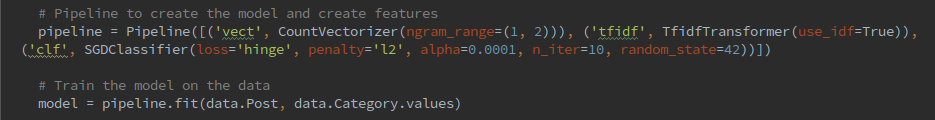
\includegraphics[width=\textwidth]{Images/Implementation/content-train}
\caption{Training the model}
\label{fig:imp-content-train}
\end{figure}

However, as well as building the model using the entire dataset, cross-validation is also implemented. Figure \ref{fig:content-cv} shows how cross-validation is performed. This is done alongside the training of the model in \emph{train.py}. The function \textit{cv\_val\_score()} is imported from scikit-learn, and handles the splitting of the dataset, and the training and testing of each model.

\begin{figure}[H]
\centering
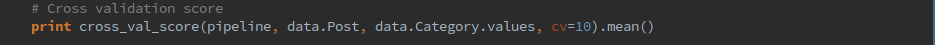
\includegraphics[width=\textwidth]{Images/Implementation/content-cv}
\caption{Cross-validating the model}
\label{fig:content-cv}
\end{figure}

The graph in figure \ref{fig:cv-results} shows the accuracy of each model for each iteration of the 10-fold cross-validation. SGD produces the best performing model, with an average accuracy of 0.606 and therefore would be a sensible choice of model for Fidelis. The SVM performs the worst, however, the accuracy of the models could be improved in the future, by fine tuning model parameters. In addition, the cross-validation is performed on full posts, and therefore the accuracy when the model is used for predicting the category of tags can be evaluated separately, when there is a sufficiently large dataset to test.

\begin{figure}[H]
\centering
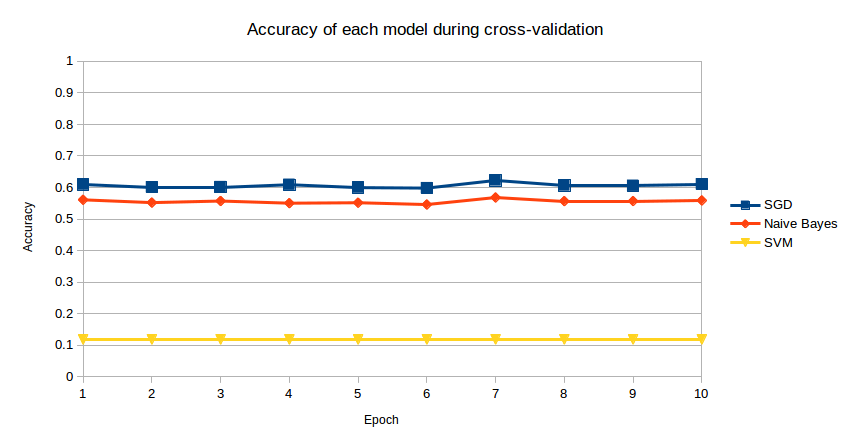
\includegraphics[width=\textwidth]{Images/Implementation/cv-results}
\caption{Cross-validation results for each model}
\label{fig:cv-results}
\end{figure}

\subsubsection{Predicting Topics}
The categories of the tag are predicted every 15 minutes by the execution of a scheduled program. This Python script, which is in figure \ref{fig:predict-tag} collects all the tags from the \emph{tags} table where the \emph{categorised} attribute is set to 0. These uncategorised tags are then passed to the imported classification model, which predicts which category the tag belongs to. Finally, the database is updated and the category-tag pairs are added to the \emph{category\_tags} table so that they can be used by the discover page. Interactions with the database are handled using a MySQL cursor from the \emph{mysql} package. The cursor is open throughout the execution of the script until it is closed at the end of the prediction process. All of the tags collected from the database are stored in a Pandas dataframe so that they can be passed to the machine learning model. Furthermore, the \emph{category.csv} file is imported, which contains the mappings from the integer values representing the categories in the trained model and the actual name of the category.

\begin{figure}[H]
\centering
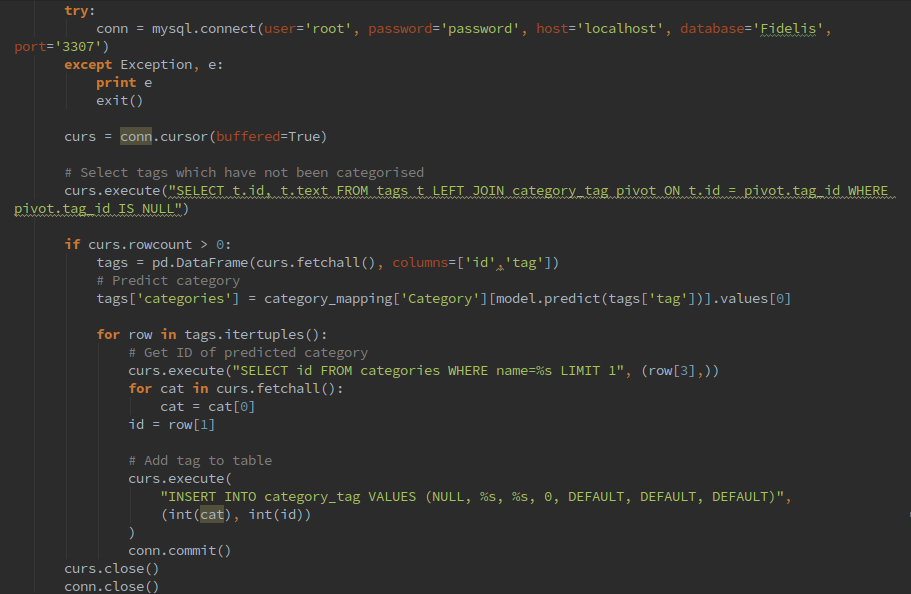
\includegraphics[width=\textwidth]{Images/Implementation/predict-tag}
\caption{Predicting the tag's category}
\label{fig:predict-tag}
\end{figure}

Post categories are predicted using the API, which makes a call to the \emph{PostController}'s \textit{predict()} function after a post has been made. As shown in figure \ref{fig:predict-api}, the function attaches the post to the tag which represents the category. Because the model used to predict the post is a Python script, the \emph{PostController} uses the $Process$ object to run the script and retrieve the predicted category which is returned by the script. After attaching the post to the tag, and thus adding the post-tag pair to the \emph{post\_tag} table, the API returns the post's category so that JavaScript can be used to update the category on the user's display. 

\begin{figure}[H]
\centering
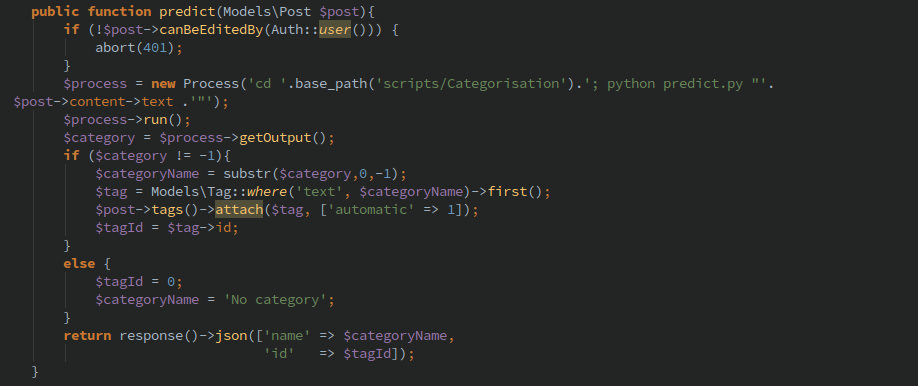
\includegraphics[width=\textwidth]{Images/Implementation/predict-api}
\caption{API controller for predicting a post}
\label{fig:predict-api}
\end{figure}

The code in figure \ref{fig:predict-post} shows the Python script which is used to predict the category of the post. As with figure \ref{fig:predict-tag}, the code is stored in the \emph{predict.py} file, but the two sections are distinguished by whether a post ID argument is passed when executing the script or not. This part of the script does not use MySQL cursors because any processing involved with the database is handled in the \emph{PostController}. 

\begin{figure}[H]
\centering
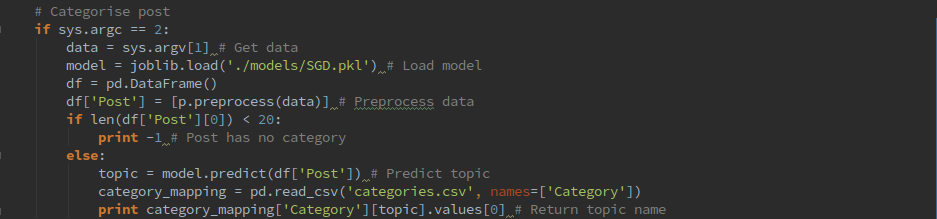
\includegraphics[width=\textwidth]{Images/Implementation/predict-post}
\caption{Predicting a post's category}
\label{fig:predict-post}
\end{figure}

Once the post has been categorised, the user would then be able to change this category in the event that the post has been misclassified. This may be the case when the post does not belong to a category, because the model will always predict that the post belongs to one of the 13 categories even if it is miscellaneous (unless the preprocessed post contains less than 20 characters). The updating of the category is performed by the API once the user has selected a new category using the Bootstrap modal shown in figure \ref{fig:category-modal}. 

\begin{figure}[H]
\centering
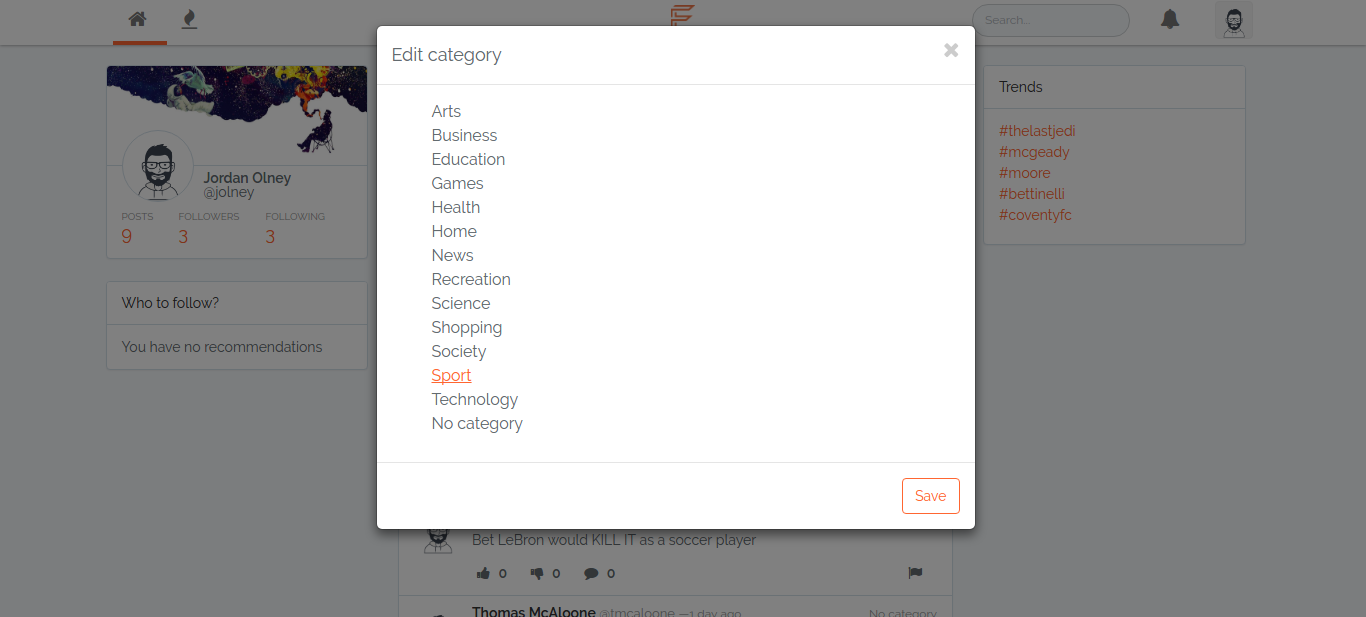
\includegraphics[width=\textwidth]{Images/Implementation/category-modal}
\caption{Modal to edit post category}
\label{fig:category-modal}
\end{figure}

The API request passes the relevant post and (new) category IDs to the \textit{editCategory()} function in the PostController, which is shown in figure \ref{fig:edit-category}. This function removes the old category from the post\_tags table and replaces it with the new one. The API then returns the new category name to the application front-end so that the changes can be reflected by the user interface. 

\begin{figure}[H]
\centering
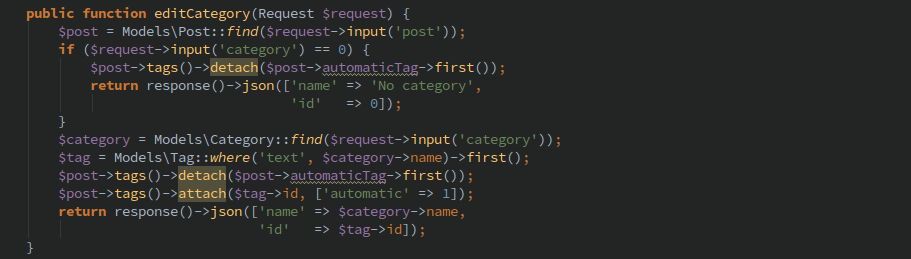
\includegraphics[width=\textwidth]{Images/Implementation/edit-category}
\caption{API controller for changing a post's category}
\label{fig:edit-category}
\end{figure}


\subsection{Content Recommendation}
Content recommendations are generated from a single Python script. It was decided to go with a single script as certain techniques are shared between user and post recommendations. The script is modularised by using functions that enable code blocks to be re-used. Python list comprehension provides a succinct way to generate lists \cite{Python:ListComprehension}, and this syntax is used throughout implementation.

Before recommendations can be made, a database connection is established using the \emph{mysql.connector} library, ``a Python driver for communicating with MySQL servers'' \cite{MySQL:MySQLConnector}. This library contains a number of useful functions for database interactions. Recommendation generation only occurs if the attempt to connect to the database is successful, otherwise, an error message is logged. This prevents erroneous system behaviour. To begin recommendations, all users are first retrieved from the database. To tailor recommendations to a specific user, user settings for how they want their recommendations to be generated are retrieved. Default settings are set for new users but these can be changed on the settings page. The settings retrieved are for recommendation preference (FOF, Explorer or Hybrid recommendations), the number of recommendations to generate, recommendation threshold (for vector similarity) and recommendation reputation. Figure \ref{fig:RecommendationSettings} shows how user settings are retrieved.


\begin{figure}[H]
\centering
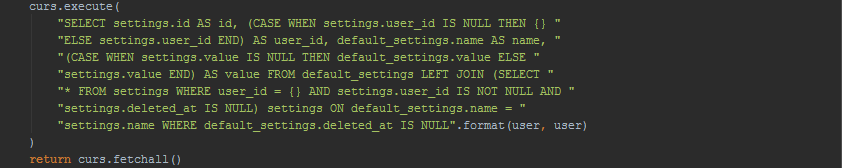
\includegraphics[width=\textwidth]{Images/Implementation/RecommendationSettings}
\caption{Query for user settings retrieval}
\label{fig:RecommendationSettings}
\end{figure}

Letting the user have control over these settings will allow them to fine-tune how they want to receive recommendations. Recommendations are generated using either FOF, Explorer or Hybrid users. The technique chosen for generation is dependent on the preference set by the user. To begin with, a query retrieving a count of the number of user recommendations already generated for the user is retrieved. New recommendations are only made if this count is less than the number of recommendations specified by the user. We will now look at how each of these techniques is implemented. Processes will be discussed for an individual user, who we will refer to as the recommendee, but each is repeated for all users stored in the database. The next two sections will look at how user and post recommendations are generated.

\subsubsection{Friend-of-a-Friend Recommendations}
FOF candidate recommendations are retrieved by first getting all users followed by the recommendee. These users are looped through, and for each of them the users they follow are collected and appended to a list. The recommendee is excluded from this list. Once this list has been generated, it is flattened to become a single list, which we will refer to as the \textit{fof\_users} list.

\paragraph{User} From this list, FOF user recommendations are chosen by converting the list to a \emph{Counter} object and picking the most common elements. The counter object was used for this purpose as it enables quick tallying \cite{Python:Counter} using the \textit{most\_common()} method. This function accepts a parameter value for the number of common elements to be returned, and by setting a value for it, we can ensure that only the number of required recommendations for the recommendee are returned. Use of the Counter object is given below:

\begin{lstlisting}[language=python]
    fof_users = Counter(fof_users).most_common(num_recommendations)
\end{lstlisting}

The reasoning for not using cosine similarity between candidate recommendations and the recommendee are given in Chapter \ref{Chapter:Design}.

\paragraph{Post} Using the same technique for post recommendations, the users in the \textit{fof\_users} list are looped through, retrieving the posts made by each of the users. For a post to suffice as a candidate recommendation for the recommendee, its reputation is compared with the reputation threshold set by the recommendee. If the reputation of the post exceeds the threshold, it is returned as one of the posts in the list of recommendations for the recommendee. Performing this check ensures again that recommendations being made are tailored to the recommendee's preferences.

\begin{figure}[H]
\centering
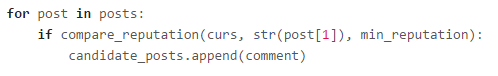
\includegraphics[width=\textwidth]{Images/Implementation/FOFPostReputation}
\caption{Code for assessing the reputation of a candidate post recommendation}
\label{fig:FOFPostReputation}
\end{figure} 

\subsubsection{Explorer Recommendations}
Explorer recommendations make use of the recommendee's `tag count vector', which is a vector representing the number of posts the recommendee has made in each of the available tags. The vector is generated by first creating a zero-filled list which has a length equal to the number of tags currently stored. Each entry in the list is a (TagID, Count) tuple. This list, which we shall refer to as the \emph{recommendee\_vector} is then sorted to determine the recommendee's favourite tags to post in. Candidate recommendations are retrieved from these tags. Currently, there is no cap on the number of tags looked at, but a cap on the number of `favourite tags' can be set once the system grows beyond what is considered small. The recommendee's favourite tags are looped through, retrieving other users posting in the same tag. This is shown in Figure \ref{fig:ExplorerFavouriteTags}.

\begin{figure}[H]
\centering
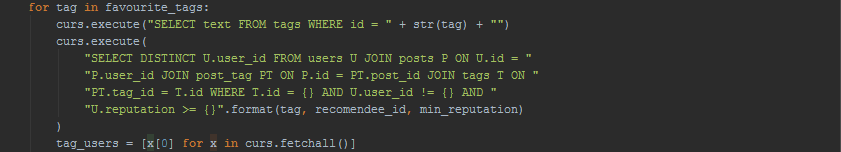
\includegraphics[width=\textwidth]{Images/Implementation/ExplorerFavouriteTags}
\caption{Code for retrieving users who post in the recommendee's preferred tags}
\label{fig:ExplorerFavouriteTags}
\end{figure}

\paragraph{User} Explorer user recommendations are assessed based on the similarity between a tag user (user also posting in one of the recommendee's preferred tags) and the recommendee. The similarity is measured using cosine similarity. SciPy provides a number of distance computation functions, one of which is the cosine distance. This is used to measure the distance between the vector generated for the tag user and the recommendee's vector. To get similarity from this, the result of this measurement is subtracted from one.

\begin{figure}[H]
\centering
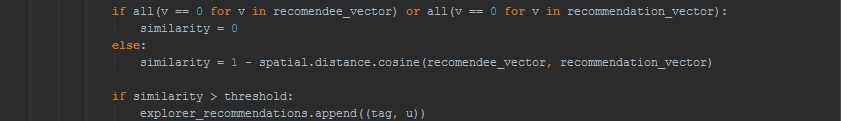
\includegraphics[width=\textwidth]{Images/Implementation/ExplorerSimilarity}
\caption{Measuring similarity between users for Explorer recommendations}
\label{fig:ExplorerSimilarity}
\end{figure}

\noindent In Figure \ref{fig:ExplorerSimilarity}, we see that we need to account for a user vector containing all zeros. This is possible for new or existing users who have made no posts. To handle such a situation, the similarity is only measured if neither of the two user vectors contains only zeros. Once similarity is measured, it is compared with the threshold for similarity set by the user. Only users with a similarity that exceeds this threshold are given as recommendations. Before the set of user recommendations is returned, its length is compared with the number of recommendations needed to provide only the required number of recommendations. 

\paragraph{Post} Similarly to post recommendations generated using the FOF technique, posts made by each of the tag users are retrieved. Only those exceeding the reputation set by the recommendee are given as recommendations. Akin to user recommendations, only the number of required recommendations are returned.

\subsubsection{Hybrid Recommendations}
Hybrid recommendations are generated by finding the intersection between the recommendations made using the FOF and Explorer recommendation methods. The Python Standard Library provides a \textit{sets} module, which can create a set of unordered, unique elements from a list \cite{Python:Sets}. Using this module, it is possible to convert the lists returned from each of the recommendation methods to sets and find the intersection between the two. We can see this in Figure \ref{fig:HybridRecommendations}.

\begin{figure}[H]
\centering
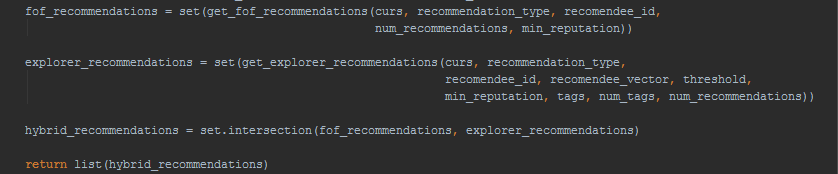
\includegraphics[width=\textwidth]{Images/Implementation/HybridRecommendations}
\caption{Generation of hybrid recommendations}
\label{fig:HybridRecommendations}
\end{figure}

\subsubsection{Default Recommendations}
In the event that all previous methods for generating recommendations fail, the script reverts to a default method that will generate generic recommendations for the recommendee. 

\paragraph{User} Default user recommendations will consist of users with the highest reputation in the system. To further filter this, only users with a reputation greater than the minimum reputation set by the user are returned.

\begin{figure}[H]
\centering
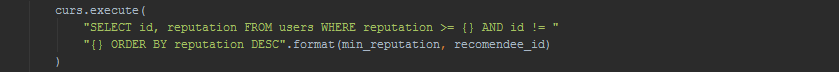
\includegraphics[width=\textwidth]{Images/Implementation/DefaultUsers}
\caption{Query for selecting most reputable users}
\label{fig:DefaultUsers}
\end{figure}

\paragraph{Post}
Similarly to users, default post recommendations are made based off the most reputable posts in the system.

\begin{figure}[H]
\centering
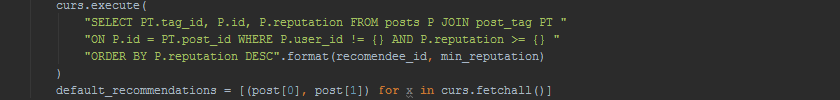
\includegraphics[width=\textwidth]{Images/Implementation/DefaultPosts}
\caption{Query for selecting most reputable posts}
\label{fig:DefaultPosts}
\end{figure}

\subsubsection{Cleaning and Saving Recommendations}
Once recommendations have been generated, they need to be cleaned. The first step in cleaning involves removing any recommendations the recommendee has not responded to. In addition to this, cleaning user recommendations consists of:
\begin{itemize}
\item Removing blocked users
\item Removing users the recommendee already follows
\item Removing the recommendee themselves
\end{itemize}

\noindent Cleaning post recommendations consists of:
\begin{itemize}
\item Removing posts made by users the recommendee has blocked
\item Removing posts the recommendee has voted on and therefore has already seen
\end{itemize}

In the case of cleaning post recommendations, posts made by the recommendee are not removed as all queries involving candidate post recommendations omit posts made by the recommendee.

Once recommendations have been cleaned, new recommendations are inserted into the relevant table. After storing the recommendations, changes made to the database must be committed using the \textit{commit()} function on the MySQL connection object.
\subsection{Reputation Scoring}
Reputation Scores are generated using two python scripts. One for reputation scoring posts and another for reputation scoring users. The scripts will each be scheduled to automatically run periodically and require no external intervention to execute. Each script will first establish a connection to the database using the mysql.connector library [39]. The library contains several functions to interact with the database. Once a connection is established, the database is queried and the results of those queries are used in the script to generate reputation scores for each post or user in the system (depending on the script). These scores are then normalised between 0 and 1 and then the database is updated with these newly calculated reputation scores using the database connection created earlier. The connection is then closed before the script terminates.

\subsubsection{Reputation Scoring for Posts}
Once a connection to the database has been established, the database must be queried to return a table with the values required to score the reputation of each post. These values are: The number of comments on the post, the number of upvotes on the post and the number of downvotes on the post. Figure \ref{fig:PostRepQuery} shows the query used to attain these values. The query selects 3 attributes from the comments table, grouped by the post id. The comments table is used because every post in the system is treated as a `root comment'. The first attribute, `comments' finds the number of entries in this table with the id of the post, subtracting 1 since the post itself must be discounted. The `upvotes' and 	`downvotes' attributes are found simply by finding those values from the comments table. Note that the query also performs the weighting needed for the summation of these attributes in the algorithm.

\begin{figure}[H]
\centering
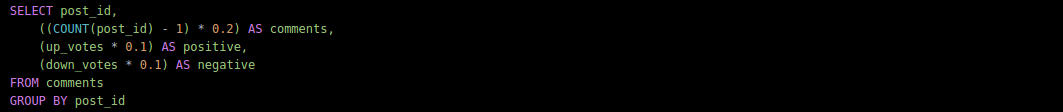
\includegraphics[height=1in]{Images/Implementation/PostRepQuery}
\caption{Query for selecting values for reputation scoring of posts}
\label{fig:PostRepQuery}
\end{figure}

Upon the conclusion of this query, the result will be a table similar to that shown in Figure \ref{fig:PostRepTable}.

\begin{figure}[H]
\centering
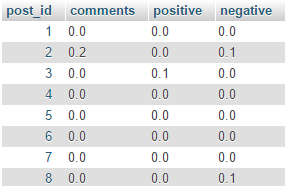
\includegraphics[height=1.5in]{Images/Implementation/PostRepTable}
\caption{Table showing example values for reputation scoring of posts}
\label{fig:PostRepTable}
\end{figure}

The python script will then iterate through each row of the result of this query. For each row, the script will perform the summation of the weighted values (comments, positive and negative) to get a reputation value. Note that the `negative' value for each post is subtracted instead of added to comply with the desired weightings. These values are all then inserted into a pandas dataframe \cite{Pandas} along with their respective post id. This is shown in Figure \ref{fig:PostRepPython1}.

\begin{figure}[H]
\centering
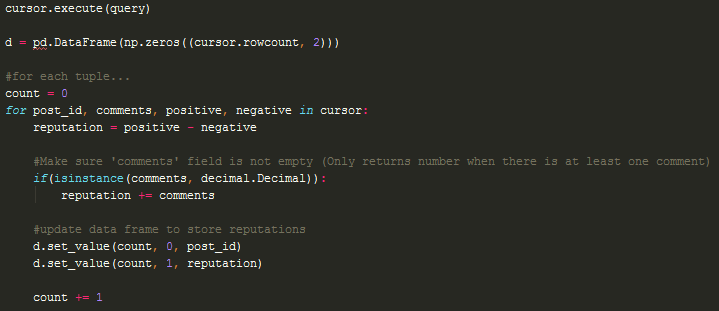
\includegraphics[width=\linewidth]{Images/Implementation/PostRepPython1}
\caption{Python code for calculating post reputation scores}
\label{fig:PostRepPython1}
\end{figure}

The script will now find the maximum and minimum reputation scores of all of the users as shown in Figure \ref{fig:PostRepPython1}. If this difference is 0, it must follow that every single post has the exact same reputation score (An unlikely scenario for the Fidelis system due to the large number of intended users). If this is the case, all of the posts will have their reputations scaled to 0. If this difference is not 0, a Python lambda function is used to normalise all reputation scores between 0 and 1. This lambda function is applied to the entire dataframe column, rather than iterating over each one individually.

\begin{figure}[H]
\centering
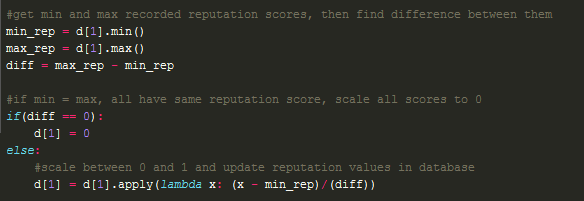
\includegraphics[width=\linewidth]{Images/Implementation/PostRepPython2}
\caption{Python code for normalising post reputation scores}
\label{fig:PostRepPython2}
\end{figure}

Finally, as shown in Figure \ref{fig:PostRepPython3}, the script runs through each row of the dataframe and updates the reputation score of each post using the final, normalised reputation score and the associated post id. This is done in the form of an SQL update query which is then committed to the database. Once each post has been assigned a new score, the database connection is terminated along with the script.

\begin{figure}[H]
\centering
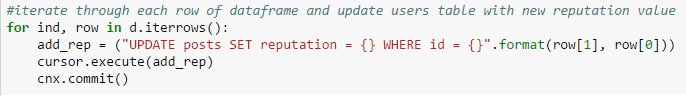
\includegraphics[width=\linewidth]{Images/Implementation/PostRepPython3}
\caption{Python code for inserting post reputation scores into the database}
\label{fig:PostRepPython3}
\end{figure}

\subsubsection{Reputation Scoring for Users}
Once a connection to the database has been established, the database must be queried to return a table with the values required to score the reputation of each user. These values are: the number of upvotes on all of the user's posts, the number of downvotes on all of the user's posts, the number of comments on all of the user's posts, the number of upvotes on all of the user's comments, the number of downvotes on all of the user's comments and the number of followers a user has. Figure \ref{fig:UserRepQuery} shows the query used to attain these values. The query selects 4 attributes from the various tables, using a number of joins. In total, the query joins together 3 separate subqueries. The first subquery finds the weighted number of upvotes on all of the user's comments and posts as well as the weighted number of downvotes on all of the user's comments. The next subquery will find the weighted number of comments on all of the users posts, where the comment isn't a `root comment' (i.e. a post) and the user id on the comment is not that of the user whose reputation is being scored. This avoids a user potentially creating many comments on their own posts simply to `boost' their reputation score.

\begin{figure}[H]
\centering
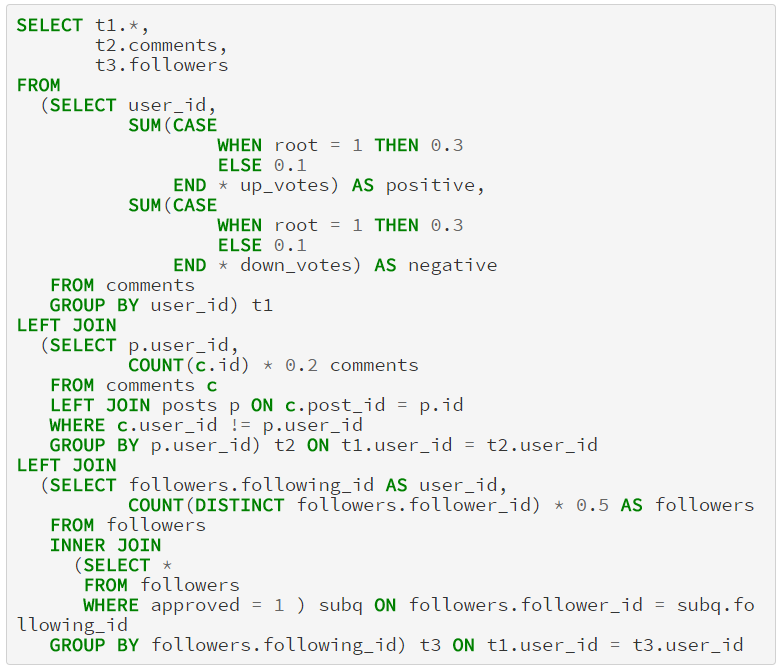
\includegraphics[height=4in]{Images/Implementation/UserRepQuery}
\caption{Query for selecting values for reputation scoring of users}
\label{fig:UserRepQuery}
\end{figure}

Upon the conclusion of this query, the result will be a table similar to that shown in Figure \ref{fig:UserRepTable}.

\begin{figure}[H]
\centering
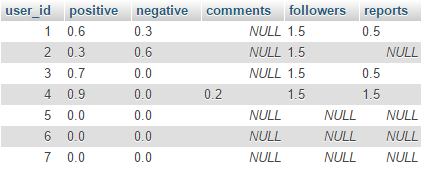
\includegraphics[height=1.5in]{Images/Implementation/UserRepTable}
\caption{Table showing example values for reputation scoring of users}
\label{fig:UserRepTable}
\end{figure}

The python script will then iterate through each row of the result of this query. For each row, the script will perform the summation of the weighted values (positive, negative, comments and followers) to get a reputation value. Note that the `negative' value for each user is subtracted instead of added to comply with the desired weightings. These values are all then inserted into a pandas dataframe \cite{Pandas} along with their respective user id. This is shown in Figure \ref{fig:UserRepPython1}.

\begin{figure}[H]
\centering
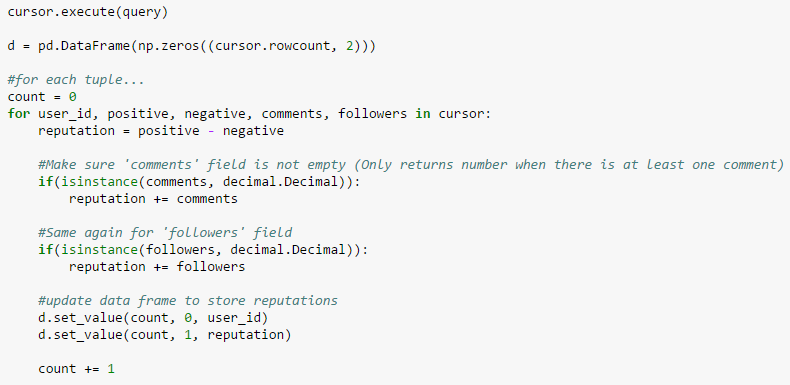
\includegraphics[width=\linewidth]{Images/Implementation/UserRepPython1}
\caption{Python code for calculating user reputation scores}
\label{fig:UserRepPython1}
\end{figure}

The script will now find the maximum and minimum reputation scores of all of the users as shown in, using the same method demonstrated for normalising the reputation scores for posts. On completion of this normalisation, every reputation score will be between 0 and 1. Finally, as shown in Figure \ref{fig:UserRepPython2}, the script runs through each row of the dataframe and updates the reputation score of each user using the final, normalised reputation score and the associated user id. This is done in the form of an SQL update query which is then committed to the database. Once each user has been assigned a new score, the database connection is terminated along with the script.

\begin{figure}[H]
\centering
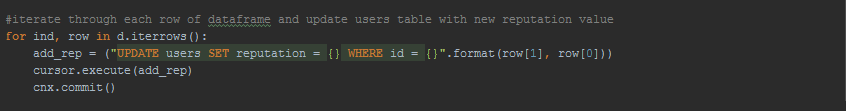
\includegraphics[width=\linewidth]{Images/Implementation/UserRepPython2}
\caption{Python code for normalising user reputation scores}
\label{fig:UserRepPython2}
\end{figure}